\section{Integracija IP jezgra sa Zynq sistemom}

PyGears i SystemVerilog implementacije predložene arhitekture su kompatibilne u
pogledu spoljnih interfejsa.
Pored toga ove implementacije su uveliko nezavisne od ciljane tehnologije za
implementaciju. \\
U ovom radu IP jezgro će biti implementirano na Zynq \gls{soc} sistemu. \\

Korišćeni DTI interfejs je kompatibilan sa AXI-Stream intefejsom, tako da je
integracija sa sistemima koji koriste druge interfejse poput Avalon-a trebala
biti jednostavna uz adaptere. \\

Preporučena je integracija IP jezgra u sistem sa procesorom, što će biti i
prikazano u ovom radu.
U ovom slučaju biće korišćen ARM Cortex-A9 procesor koji se može naći kao Hard
IP jezgro unutar Zynq SoC platforme kompanije Xilinx. \\

\subsection{Zynq}

Zynq se sastoji od \gls{ps} sistema i \gls{pl} sistema.
PS sistem je sačinjen od već pomenutog ARM Cortex-A9 \gls{APU} procesora.
Dok PL sistem predstavlja \gls{fpga} programabilnu logiku Artix-7 familije. \\

Komunikacija između PL i PS sistema se obavlja preko \gls{axi} interfejsa,
interapt pinova ili \gls{emio} pinova.\\

ARM procesor ima mogućnost povezivanja eksterne \gls{ddr} memorije preko
internog DDR kontrolera.
Preko ovog kontrolera pristup memoriji ima i PL sistem. \\
Zynq SoC ima mogućnost pokretanja GNU/Linux operativnog sistema.

\newpage

\subsection{Predloženi blok dijagram sistema}

U nastavku je prikazan okviran blok dijagram povezivanja projektovanog IP jezgra
sa procesorskim sistemom. \\
Na slici su izostavljene interkonekcijske komponente, generatori reset i clk signala,
DDR konekcije itd... \\

\begin{figure}[H]
  \centering
  \resizebox{1\textwidth}{!}{%
    \pgfdeclarelayer{background1}
\pgfdeclarelayer{background2}
\pgfdeclarelayer{foreground}
\pgfsetlayers{background1, background2,main,foreground}

\tikzstyle{cloud1} = [draw=black, thick, fill=red!20, minimum height = 1em]
\tikzstyle{block_l} =[draw, text centered, fill=blue!15, minimum width=2.5cm, minimum height=2.5cm]
\tikzstyle{block_m} =[draw, text centered, fill=blue!15, minimum width=2.0cm, minimum height=1.0cm]
\tikzstyle{block_s} =[draw, text centered, fill=blue!15, minimum width=2cm, minimum height=1.5cm]
\tikzstyle{line} = [draw, line width = 0.05cm, arrows={-Triangle[length=0.2cm]}]

\tikzstyle{dreg} = [draw, text centered, fill=blue!15, minimum width = 1.5cm,
minimum height=1.5cm]

\tikzstyle{square} = [draw, thick, fill=blue!15, circle, minimum size = 1cm, node distance = 2cm]
\tikzstyle{mult} = [draw, thick, fill=blue!15, circle, minimum size = 1cm ,node distance = 2cm]
\tikzstyle{sum} = [draw, thick, fill=blue!15, circle, minimum size= 1cm, node distance = 2cm]

\begin{tikzpicture}[thick]

  \node [block_l, fill=red!20] (csc_cls) {\textbf{\large cascade\_classifier}};
  \node [coordinate, left = 0cm of csc_cls] (csc_cls_in){};
  \node [coordinate, left = 2cm of csc_cls_in] (ii_in){};
  \node [coordinate, above right = -0.5cm and 0cm of csc_cls] (csc_cls_out){};
  \node [coordinate, below right = -0.5cm and 0cm of csc_cls] (csc_cls_irq){};
  \node [coordinate, right = 1cm of csc_cls_irq] (csc_cls_irq1){};

  \node [block_l, fill=red!20, below = 2cm of csc_cls] (dm_cmd) {\textbf{\large dm\_cmd}};
  \node [coordinate, below left = 0 and -0.5cm of dm_cmd] (dm_cmd_in){};
  \node [coordinate, below right = 0 and -0.5cm of dm_cmd] (dm_cmd_irq_out){};
  \node [coordinate, above right = 0cm and -0.5cm of dm_cmd] (dm_cmd_irq_in){};
  \node [coordinate, above = 1cm of dm_cmd_irq_in] (dm_cmd_irq_in1){};
  \node [coordinate, left = 0cm of dm_cmd] (mm2s_cmd){};
  \node [coordinate, right = 0cm of dm_cmd] (s2mm_cmd){};

  \node [block_l, below = 2cm of dm_cmd] (apu) {\textbf{\large APU}};
  \node [coordinate, above left = 0cm and -0.5cm of apu] (apu_cmd){};
  \node [coordinate, above right = 0cm and -0.5cm of apu] (apu_irq){};
  \node [coordinate, left = 0cm of apu] (apu_mm2s){};
  \node [coordinate, right = 0cm of apu] (apu_s2mm){};

  \node [block_l, right = 3cm of csc_cls] (s2mm) {\textbf{\large dm\_s2mm}};
  \node [coordinate, right = 0cm of s2mm] (s2mm_out){};
  \node [coordinate, right = 1cm of s2mm] (s2mm_out1){};
  \node [coordinate, above left = -0.5cm and 0cm of s2mm] (s2mm_in){};
  \node [coordinate, below left = -0.5cm and 0cm of s2mm] (s2mm_cfg){};
  \node [coordinate, left = 1cm of s2mm_cfg] (s2mm_cfg1){};


  \node [block_l, left = 2cm of csc_cls] (mm2s) {\textbf{\large dm\_mm2s}};
  \node [coordinate, above left = -0.5cm and 0cm of mm2s] (mm2s_in){};
  \node [coordinate, left = 2cm of mm2s_in] (mm2s_in1){};
  \node [coordinate, below left = -0.5cm and 0cm of mm2s] (mm2s_cfg){};
  \node [coordinate, left = 1cm of mm2s_cfg] (mm2s_cfg1){};
  \node [coordinate, right = 0cm of mm2s] (mm2s_out){};

  %% group %%
 \begin{pgfonlayer}{background1}
   \node[inner sep=20pt, fill=yellow!25, rounded corners, draw, thick,fit=(csc_cls) (s2mm_out1) (mm2s_in1) (dm_cmd) (mm2s) (s2mm) (apu)] (system) {};
  \node[above left] at (system.south east) {\huge \textbf{SoC}};
\end{pgfonlayer}


  % arrows
  \path [line] (csc_cls_out) node[transition, yshift=+0.3cm, xshift=+1.3cm] {detect\_addr}  -- (s2mm_in);
  \path [line] (mm2s_out) -- (csc_cls_in) node[transition, yshift=+0.3cm, xshift=-0.8cm] {img\_in}  ;
  \path[line] (csc_cls_irq) node[transition, yshift=+0.3cm, xshift=+0.6cm] {irq}  -- (csc_cls_irq1) |- (dm_cmd_irq_in1) -- (dm_cmd_irq_in);

  \path [line] (s2mm_cmd) node[transition, yshift=+0.3cm, xshift=+1.0cm] {s2mm\_cfg} -| (s2mm_cfg1) -- (s2mm_cfg);
  \path [line] (mm2s_cmd) node[transition, yshift=+0.3cm, xshift=-1.0cm] {mm2s\_cfg} -| (mm2s_cfg1) -- (mm2s_cfg);

  \path[line] (s2mm_out) node[transition, yshift=+0.3cm, xshift=+0.8cm] {s2mm}  -- (s2mm_out1) |- (apu_s2mm);

  \path[line] (apu_mm2s) node[transition, yshift=+0.3cm, xshift=-0.8cm] {mm2s} -| (mm2s_in1) -- (mm2s_in);

  \path[line] (apu_cmd) node[transition, yshift=+0.5cm, xshift=-1.0cm] {apu\_cmd}  -- (dm_cmd_in);

  \path[line] (dm_cmd_irq_out) node[transition, yshift=-0.5cm, xshift=+0.4cm] {irq}  -- (apu_irq);


\end{tikzpicture}
  }
  \caption{Okviran blok dijagram sistema.}
  \label{system_bd_approx}
\end{figure}

Blokovi obojeni crvenom bojom su projektovani u okviru ovog rada.
Blokovi obojeni plavom bojom su standardne komponente i mogu se naći u okviru
softverskog alata od proizvođača korišćenog SoC-a. \\

Kako je već rečeno spoljni interfejsi \textbf{cascade\_classifier} IP jezgra su
Streaming tipa.
Streaming interfejsi nemaju informaciju o adresi, tako da sa njima nije
moguće adresirati podatak iz DDR memorije preko DDR kontrolera. \\

Komponente dm\_s2mm i dm\_mm2s su Data Mover-i, koji pretvaraju Streaming interfejs u \gls{mm}
interfejse.
Kako Streaming interfejs prenosi samo podatak i nema informaciju o
adresi, potrebno je proslediti adresu i broj podataka preko posebnog komandnog
interfejsa, na ovoj slici to su s2mm\_cfg i mm2s\_cfg.\\

Glavno IP jezgro nema koristi od informacije sa koje adrese dolazi slika i na
kojoj adresi se smeštaju rezultati, pa je zato za generisanje komande za Data Mover
komponente zadužen dm\_cmd.\\
Komponenta dm\_cmd od procesora dobija adresu bafera slike i rezultata iz eksterne DDR
memorije i na osnovu toga generiše komande za Data Mover-e. \\
Adrese i broj podataka procesor šalje preko apu\_cmd interfejsa. \\

Nakon konfigurisanja Data Mover-a prvo će sa radom početi dm\_mm2s Data Mover,
koji će poslati zahtev za sliku DDR kontroleru i pročitane podatke proslediti
glavnom IP jezgru na obradu.
Nakon popunjavanja IMG RAM memoriju unutar glavnog IP jezgra, jezgro počinje
obradu slike. \\

Ukoliko dođe do detekcije objekta na nekoj koordinati, ta koordinata će biti
poslata preko dm\_s2mm Data Mover-a u određenu lokaciju za smeštanje rezultata u
okviru eksterne DDR memorije. \\

Nakon završetka obrade trenutne slike aktiviraće se irq signal koji označava
interrupt za procesor.
Glavno IP jezgro će držati aktivnim ovaj signal samo jedan takt, dok će se taj
signal sačuvati u registru u okviru dm\_cmd jezgra i biće prosleđen na izlazni
irq signal povezan sa procesorom. \\
Nakon detekcije interapt signala od strane procesora, poslaće se zahtev za reset
ovog registra preko apu\_cmd interfejsa.
Sam interapt signal procesoru signalizira da može početi sa pripremanjem sledeće
slike.
Nakon smeštanja naredne slike u bafer, procesor ponovo šalje zahtev za obradu
slike preko apu\_cmd interfejsa. \\

Procesor pored slanja komande IP jezgru treba da preuzme sliku sa kamere ili
učita iz fajla, zatim je konvertuje u grayscale reprezentaciju.
Nakon prihvatanja rezultata detekcije procesor može koristiti dobijene
koordinate za željeni zadatak. \\
Broj primena algoritama za detekciju objekata je ogroman i od korisnika zavisi
dalja implementacija softvera.
Rad IP jezgra u ovom radu je demonstriran iscrtavanjem pravougaonika na
pozicijama detektovanih objekata i prikazivanjem slike sa iscrtanim
pravougaonicima na HDMI monitor. \\

\newpage

\subsection{Implementirani sistem na Zynq SoC}

U ovom radu sistem je implementiran na Zynq-7020 SoC.
Korišćena je ZTurn\cite{zturn} ploča firme MYiR.
Ova ploča se sastoji od Zynq-7020 čipa, 1GB eksterne DDR3 memorije, \gls{hdmi}
kontroler i konektor, tasteri i \gls{led} za testiranje, g-senzor, temperaturni
senzor, buzzer, flash memorija, SD card socket, Gig ethernet, JTAG, USB, CAN itd...
Što se može videti na sledećoj slici. \\

\begin{figure}[H]
  \centering
  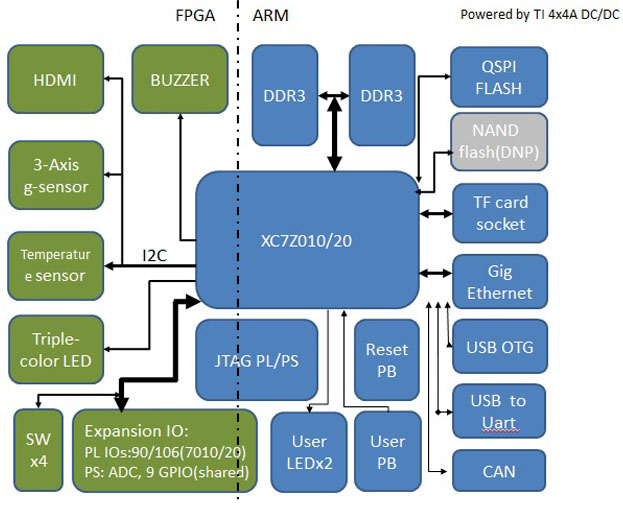
\includegraphics[width=0.65\linewidth]{images/zturn.jpg}
  \caption{Zturn ploča\cite{zturn}}
  \label{zturn_bd}
\end{figure}



Od eksternih periferija u ovom projektu korišćeni su SD kartica, Ethernet, HDMI,
USB i DDR memorija.
Procesor pokreće Arch Linux ARM\cite{arch} operativni sistem, a komunikacija sa IP jezgrom je
odrađena preko napisanog Linux Kernel Drivera i korisničke aplikacije. \\

Na sledećoj strani prikazan je blok dijagram Vivado integratora implementiranog
sistema. \\
Može se primetiti da pored komentarisanih komponenti za povezivanje procesora sa
IP jezgrom, na blok dijagramu se nalazi i Video kontroler pod nazivom
hdmi\_core.
Ovo jezgro se koristi za slanje sadržaja framebuffer-a Linux Kernel-a na
eksterni HDMI kontroler, u cilju grafičkog interfejsa korisničke aplikacije. \\
IP jezgro je povezano sa AXI stream periferija preko axi\_to\_dti i cast blokova,
ovi blokovi prilagođavaju DTI EOT signal sa AXI TLast signalom koji označavaju
kraj transakcije. \\
Ulazni EOT signal označava kraj upisa u IMG RAM memoriju, dok izlazni EOT signal
signalizira Data Moveru da je završena transakcija i može upisati baferovane
podatke u DDR. \\

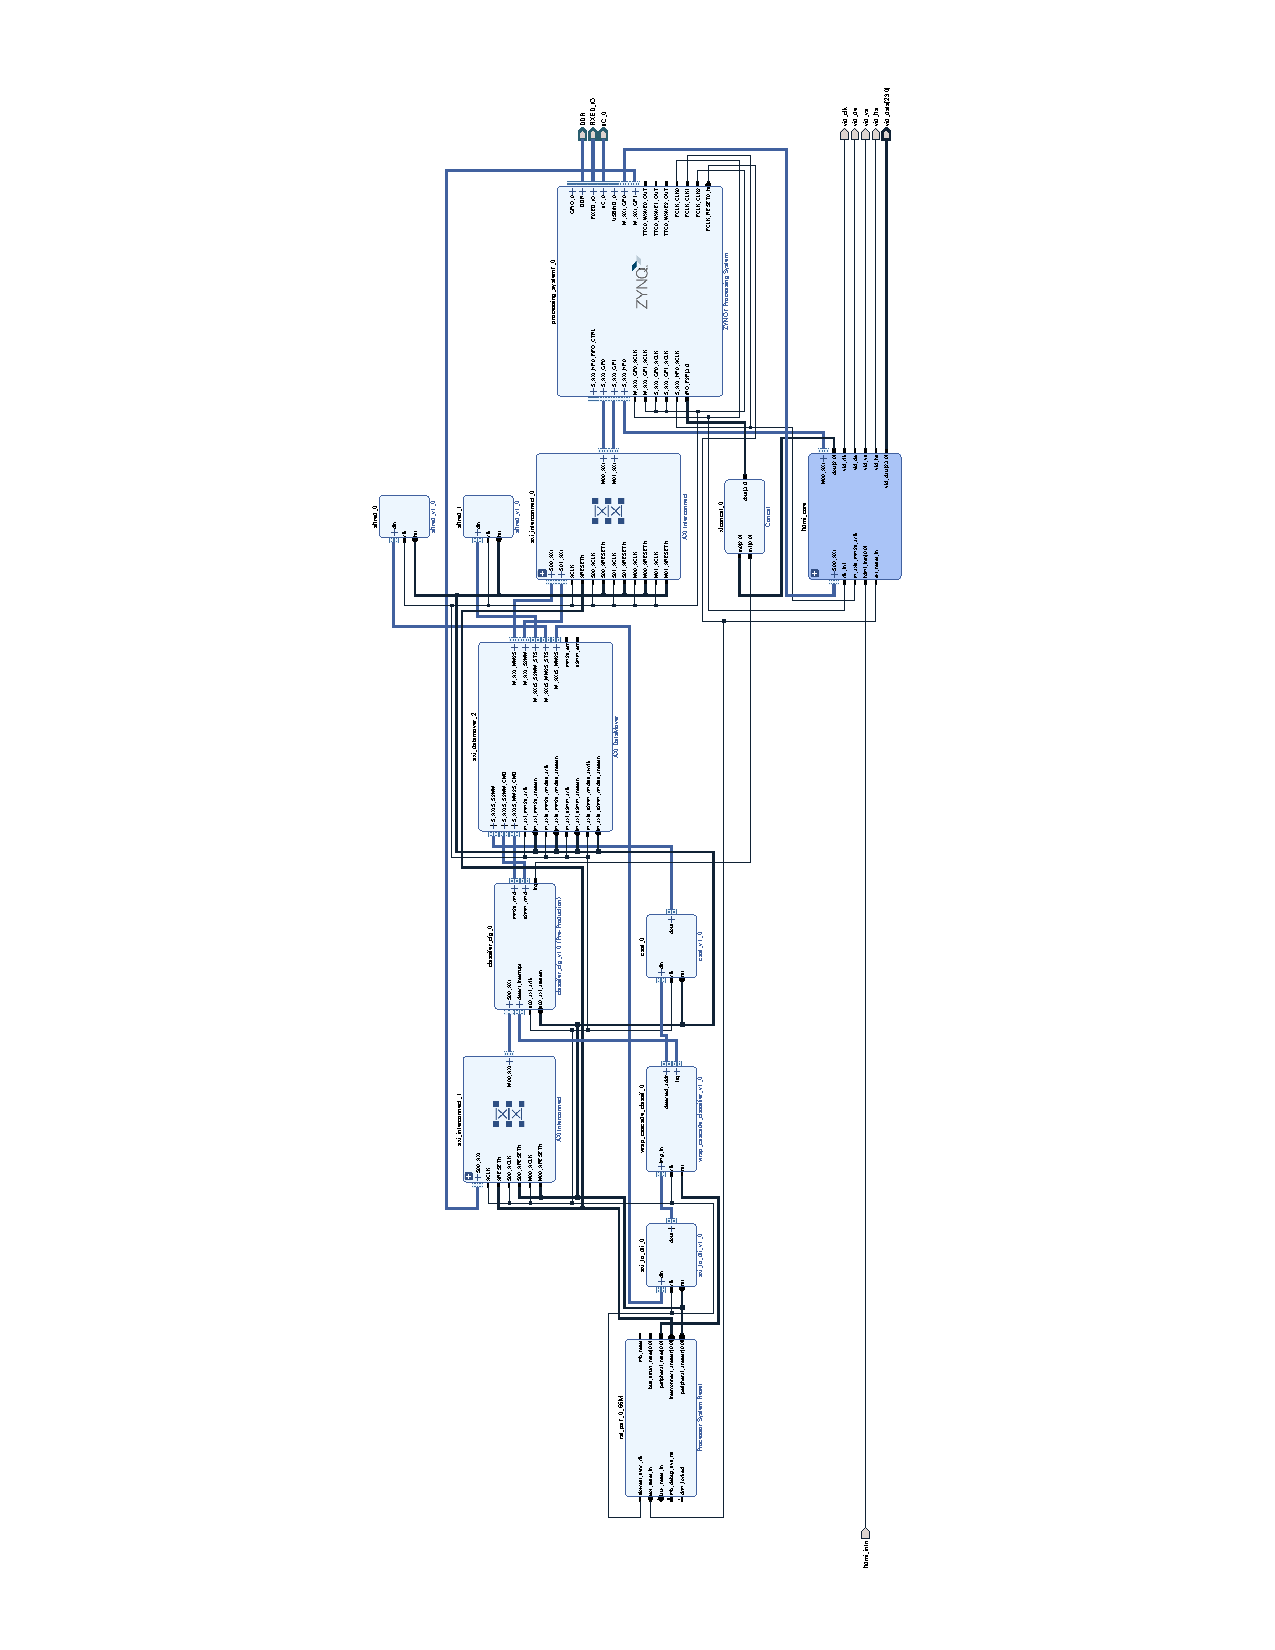
\includepdf[pages=-,pagecommand={},width=1.6\textwidth, height=1.2\textheight]{images/system_bd.pdf}


\subsection{Rezultati implementacije sistema}

\subsubsection{Sinteza i implementacija hardvera}
FPGA čipovi se sastoje od velikog broja programabilnih primitivnih blokova i
mreže za rutiranje.
Ove blokove je potrebno konfigurisati i međusobno ih povezati kako bi se dobila
željena funkcionalnost.
Kako se tipični dizajnovi koji ciljaju FPGA čipove sastoje od desetina hiljada
LUT-ova i ostalih komponenti, ovaj korak nije moguće odraditi ručno.
Sintezu i implementaciju digitalnog hardvera je jedino moguće uraditi pomoću
automatskog alata. \\

Proizvođači FPGA čipova uglavnom imaju svoj softverski alat za obavljanje ove
radnje.
Tako u slučaju Xilinx FPGA čipova potrebno je koristiti Vivado.\\

Prilikom sinteze hardvera alat hijerarhijski struktruirane HDL modele izravna i
napravi model sa jednakom hijerarhijom sačuvan u formatu netliste.
Tokom sinteze se rade i razne optimizacije poput deljenja funkcionalnih resursa,
logička minimizacija, optimizacija mašina stanja itd...
Konačno alat za sintezu može mapirati komponente generisane netliste u
primitivne blokove ciljane FPGA arhitekture, tzv Technology Mapping. \\
Nakon koraka sinteze moguće je proceniti koliko će se hardverskih primitivnih
blokova koristiti u konačnoj hardverskoj implementaciji. \\
Na osnovu toga se može zaključiti da li implementirani hardver zadovoljava
ograničenja potrošnje resursa. \\

Nakon sinteze hardvera potrebno je odraditi Place and Route komponenti na
željenom FPGA čipu.
To je takođe moguće odraditi automatskim alatom.
Nakon ovog koraka moguća je procena vremenskih karakteristika implementiranog
hardvera.
Pošto su poznata kašnjenja primitivnih blokova i moguća je estimacija kašnjenja
mreže za rutiranje može se proceniti da li će dizajn zadovoljavati vremenska
ograničenja. \\
Takođe moguće je proceniti i potrošnju konačne implementacije. \\
Konačno potrebno je generisati Bitstream fajl kojim će se konfigurisati FPGA
čip. \\

Pored zvaničnih alata za sintezu i implementaciju digitalnog hardvera na FPGA
čipovima, postoje i alternativna Open Source rešenja.
Problem sinteze rešava alat pod nazivom yosys\cite{yosys}, ovaj alat je brži od
zvaničnih alata za sintezu, uz to u nekim slučajevima generiše optimalniji
hardver, dok je manje efikasan u mapiranju hardvera na tehnologiju. \\
Za Place and Route može se koristiti nextpnr\cite{nextpnr}.
Pored toga postoji projekat SymbiFlow\cite{SymbiFlow} koji nastoji da poveže sve
ove alate i obezbedi jedinstveni alat za implementaciju digitalnog hardvera na
FPGA čipove nezavisno od proizvođača.
Veliki problem u ovom projektu predstavlja što FPGA proizvođači ne objavljuju
javno arhitekturu čipova i format Bitstream-a, pa se do ovih informacija mora
doći reverznim inženjeringom. \\

\newpage

\subsubsection{Analiza potrošnje hardverskih resursa}

U narednoj tabeli biće prikazano zauzeće hardverskih resursa u slučaju PyGears
implementacije.
Biće prikazana potrošnja samo glavnog IP jezgra i ukupnog sistema. \\

\newcolumntype{P}[1]{>{\centering\arraybackslash}p{#1}}
\begin{center}
  \centering
  \captionof{table}{Hardverski resursi nakon sinteze PyGears implementacije}
  \begin{tabular}{| P{3cm} | P{3cm} | P{3cm} | P{3cm} | P{3cm} | P{3cm} |}
    \hline
    Name  & LUT & FF & BRAM & DSP  \\ \hline
    Total & 14,259 (27\%) & 14,033 (13\%) & 47.5 (34\%) & 7 (3\%)  \\ \hline
    Cascade Classifier & 6,216 (12\%) & 2,252 (2\%) & 35 (25\%) & 7 (3\%) \\ \hline
  \end{tabular}
\end{center}

Nakon implementacije dobijaju se oko 10\% niže brojke za LUT i FF komponente. \\
Kao što se može videti najkritičniji deo ovog IP jezgra je broj korišćenih BRAM
komponenti što je bilo i očekivano na osnovu analize predložene arhitekture. \\
Može se videti da je projektovano jezgro veoma efikasno u pogledu ostalih
hardverskih resursa i ostaje prostora za ubrzanje dodavanjem hardverskih
resursa, odnosno paralelizma. \\

U nastavku je data tabela zauzeća hardverskih resursa u slučaju SystemVerilog
implemtacije iste arhitekture. \\

\newcolumntype{P}[1]{>{\centering\arraybackslash}p{#1}}
\begin{center}
  \centering
  \captionof{table}{Hardverski resursi nakon sinteze SystemVerilog implementacije}
  \begin{tabular}{| P{3cm} | P{3cm} | P{3cm} | P{3cm} | P{3cm} | P{3cm} |}
    \hline
    Name  & LUT & FF & BRAM & DSP  \\ \hline
    Total & 9,648 (18\%) & 13,875 (13\%) & 53.5 (38\%) & 15 (7\%)  \\ \hline
    Cascade Classifier & 1,605 (3\%) & 2,094 (2\%) & 41 (29\%) & 15 (7\%) \\ \hline
  \end{tabular}
\end{center}

Kao što je i očekivano SystemVerilog verzija troši manje hardverskih resursa.\\
Dodatni hardverski resursi u slučaju PyGears implementacije se uglavno ogledaju
u dodatnim LUT-ovima i FF-ovima.
Ovi LUT-ovi i FF-ovi implementiraju sinhronizaciju i handshaking u
okviru PyGears dizajna.
Kao što se može videti postoji razlika između potrošnje DSP blokova i BRAM
memorija, ove komponente uglavnom se koriste prilikom implementacije aritmetike
i memorije potrebne za samu funkcionalnost dizajna, a ne za implementaciju
sinhronizacionih komponenti.\\

Prilikom sinteze alat može odlučiti na osnovu širina magistrala da li će
aritmetičku operaciju implementirati kao DSP blok, pomoću LUT-ova ili drugih komponenti, u ova dva
slučaja zbog razlike u širinama internih signala alat za sintezu je istu
komponentu početne arhitekture implementirao na različite načine.
Tada se može desiti da su neka množenja i sabiranja u PyGears verziji
implementirana pomoću LUT-ova, dok su neke RAM ili ROM memorije implementirane
kao FF ili distribuirani RAM-ovi. \\

Pored toga u PyGears verziji se često dodaju redundantne sinhronizacione
komponente.
Primer toga je kada se iz istog izvora razdvaja signal u dve grane, pa se ti
signali dalje ``broadkastuju'' na više mesta, u ovoj situaciji određen broj dodatnih LUT-ova i
FF-ova se može ukloniti prilikom sinteze.
Nažalost zbog prilično jedinstvenog slučaja Vivado ne vrši ovu
optimizaciju, usled čega konačna implementacija rezultuje u značajnom povećanju
potrošenih hardverskih resursa.\\

Ova optimizacija je za potrebe PyGears-a dodata u Yosys open source alat za
sintezu.
Ova tvrdnja najlakše se može videti na primeru CORDIC IP jezgra.
Čista Verilog verzija CORDIC IP jezgra je sintetisana pomoću Vivado alata i
dobijeno je oko 700 LUT-ova i 800 FF-ova.
Nakon toga implementirano je isto IP jezgro u PyGears-u, gde je nakon sinteze u
Vivadu dobijeno zauzeće od 2400 LUT-ova i 1100 FF-ova. \\
Dok je u slučaju prvobitne sinteze pomoću Yosys alata pa nakon toga Vivada
dobijeno oko 800 LUT-ova i 900 FF-ova.
Kao što se može videti optimizacioni korak u Yosys sintezi značajno može
smanjiti broj hardverskih resursa i PyGears metodologija se značajno oslanja na
kvalitetan alat za sintezu. \\
Iako je ovo slučaj, u ovom projektu nije korišćen Yosys za sintezu.


\subsubsection{Analiza vremenskog izveštaja i Timing Closure}

Frekvencija takta je bitna stavka, što većom frekvencijom taktujemo IP jezgro
brzina obrade slike će biti brža.
Naravno postoji ograničenje maksimalne frekvencije koja se može postići.
Ovo ograničenje postoji zbog vremena propagacije signala kroz logičke blokove i mreže za rutiranje unutar FPGA čipa.
Izlazni signali flip flopova prolaze kroz kombinacionu logiku i dolaze do ulaza
sledećeg flip flopa, kašnjenje ove putanje mora biti kraće od periode takta uz
dodatan uticaj Setup i Hold vremena flip flopova.

\begin{figure}[H]
  \centering
  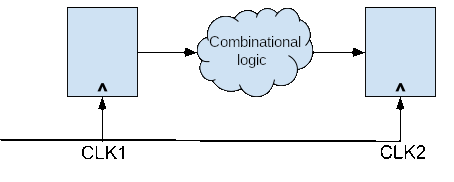
\includegraphics[width=0.55\linewidth]{images/comb.png}
  \caption{Kašnjenje kombinacione logike}
  \label{comb_logic}
\end{figure}

Mreža kombinacione logike predstavljena oblačićem može imati značajno vreme
propagacije.
Jedan od načina da se vreme propagacije smanji je ubacivanjem registara unutar
kombinacione mreže, odnosno presecanje kombinacione putanje. \\
To je ujedno i najčešća tehnika ubrzavanja dizajna u krajnjoj fazi i
zadovoljavanja vremenskih ograničenja dizajna, takozvani Timing Closure. \\

\newpage

Nakon podešavanja takta na 47MHz i pokretanja implementacije može se videti da
su vremena zadovoljena za odabrani takt. \\
Empirijski se može zaključiti da frekvencija sistema srednje veličine
implementiranog na Zynq-7020 čipu može dostići brzine oko 110MHz, na osnovu
čega možemo zaključiti da se u ovom slučaju mogu postići bolji
rezultati. \\
Na slici ispod su prikazane najkritičnije putanje u okviru dizajna. \\

\begin{figure}[H]
  \centering
  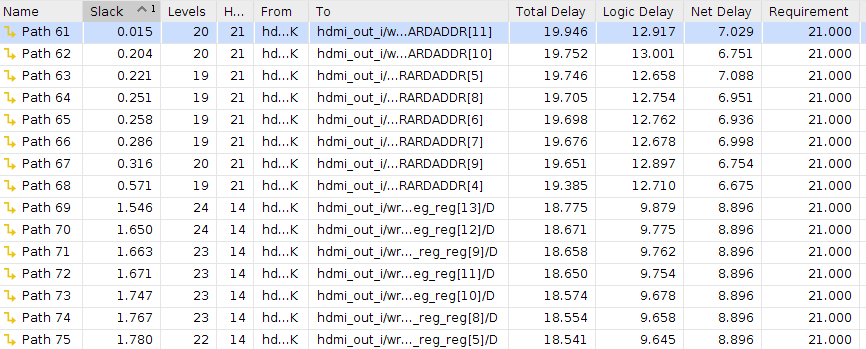
\includegraphics[width=1\linewidth]{results/implementation/pygears_slow/timing.png}
  \caption{Vremenski izveštaj pre skraćivanja kombinacionih putanja}
  \label{slow_time}
\end{figure}

Takođe može se i primetiti da je Logic Delay koji predstavlja vreme propagacije
kroz kombinacionu logiku veće od Net Delay-a koji predstavlja vreme
propagacije kroz mrežu za rutiranje.
Na Net Delay se ne može mnogo uticati i uveliko zavisi od kvaliteta korišćenog
FPGA čipa. \\

Može se primetiti veliko odstupanje između prvih desetak najkritičnijih putanja,
kao i da su putanje koje imaju Logic Delay od približno 13ns grupisane u okviru
jednog interfejsa.
To je znak da postoje putanje koje imaju značajno duže vreme propagacije od
ostatka sistema, pa je njih potrebno ubrzati. \\
Pomoću Vivado alata moguće je identifikovati putanju propagacije kritičnih
putanja i odlučiti gde bi se kombinaciona putanja mogla prekinuti i ubaciti
registar.
Ovo je dugotrajan proces i mora se raditi iz više iteracija, nakon svakog
ubacivanja registara mora se verifikovati funkcionalna ispravnost sistema, zatim
se ponovo pokreće implementacija. \\
U svakoj narednoj iteraciji sve je teže uočiti kritične putanje. \\

\newpage

PyGears dodatno olakšava proces skraćivanja kombinacionih putanja jednostavnim
ubacivanjem registara u dizajn što je prikazano na sledećem primeru. \\

\begin{code}[H]{python}{PyGears implementacija stddev komponente}{gear_example1}
from pygears import gear
from pygears.typing import Queue, Uint
from .frame_sum import frame_sum
from pygears.lib.rom import rom
from pygears.lib import dreg as dreg_sp

@gear
def stddev(ii_s: Queue[Uint['w_ii'], 2],
           sii_s: Queue[Uint['w_sii'], 2], *,
           casc_hw):

    ii_sum = ii_s | frame_sum | dreg_sp
    ii_sum_squared = ii_sum[0] * ii_sum[0]

    sii_sum = sii_s | frame_sum | dreg_sp
    sii_mult1 = sii_sum[0] * (casc_hw.frame_size[0] - 1)
    sii_mult2 = sii_mult1 * (casc_hw.frame_size[1] - 1)

    sub_s = sii_mult2 - ii_sum_squared

    sqrt_addr = sub_s >> casc_hw.sqrt_shift | Uint[8]

    stddev_res = sqrt_addr | rom(
        data=casc_hw.sqrt_mem, dtype=Uint[casc_hw.w_sqrt])

    return stddev_res
\end{code}

U kodnom segmentu iznad u liniji 5 importuje se gear dreg koji predstavlja
registar i lokalno se naziva dreg\_sp.
Ovo može biti koristan detalj jer pomaže u boljoj distinkciji između registara
koji su prisutni funkcionalno i onih koji su ubačeni radi skraćivanja
kombinacionih putanja. \\
U linijama 12 i 15 može se videti skraćivanja kombinacione putanje posle
frame\_sum gear-a ubacivanje dreg\_sp gear-a. \\

Dodatna prednost PyGears-a u ovoj situaciji je činjenica da se ubacivanjem
registara unutar dizajna ne može izgubiti funkcionalna korektnost sistema.
Iako se ne može izgubiti funkcionalna korektnost, nasumičnim ubacivanjem
registara se može pogoršati vremenske performanse.
Prilikom ubacivanja registara može doći do gubljenja balansa između dve
paralelne grane, pa će jedan podatak uvek kasniti jedan takt do sinhronizacionog
gear-a u odnosu na drugu granu, usled čega će se na izlazu sinhronizacionog
gear-a pojaviti neželjeni takt pauze.
Pažljivom analizom paralelnih grana i sinhronizacionih tačaka, moguće je
balansirati grane dodavanjem dodatnog registra u nebalansiranoj grani. \\

Konačno nakon skraćivanja kombinacionih putanja dostignuta je frekvencija takta
od 100MHz.\\
Pored skraćivanja kombinacionih putanja dodatno je uključena i
Performance ExplorePostRoutePhysOpt strategija za implementaciju u okviru
Vivado alat, ova strategija će učiniti da vreme implementacije traje duže, ali
će se kao rezultat dobiti implementacija sa boljim vremenskim karakteristikama,
ponekad sa cenom dodatnih hardverskih resursa. \\

Kao što se može videti dostignuto je više nego duplo ubrzanje sistema ovom tehnikom. \\
Treba napomenuti da je u RTL metodologiji preporučljivo voditi računa o
kombinacionim putanjama u ranijim fazama implementacije, dok je zbog lakog
ubacivanja registara u kasnijim fazama dizajna u PyGears metodologiji
pogodniji ovakav pristup. \\

\begin{figure}[H]
  \centering
  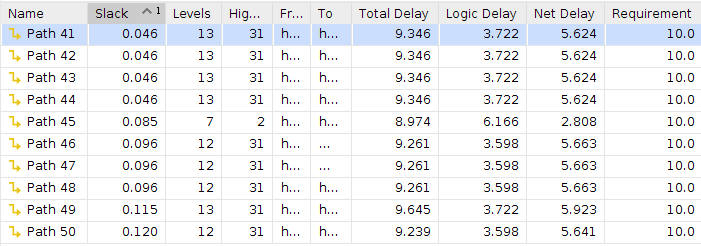
\includegraphics[width=1\linewidth]{results/implementation/pygears_fast/timing.png}
  \caption{Vremenski izveštaj posle skraćivanja kombinacionih putanja}
  \label{slow_time}
\end{figure}

Može se primetiti da je dostignuto ogromno skraćenje Logic Delay vremena, a
može se  primetiti i da je Net Delay značajno skraćen to je verovatno rezultat
lakšeg zadatka za Place and Route alat nakon ubacivanja registara. \\
Na slici je prikazano 10 kombinacionih putanja u prošlom slučaju smo primetili
veliku razliku ukupnog kašnjenja u istom broju putanja, u ovom slučaju ne bismo
primetili veliku razliku u totalnom kašnjenju čak i kod prvih 100 kritičnih
putanja, to je pokazatelj da se dolazi do granica mogućnosti ubrzavanja sistema
ovim pristupom. \\
U tom trenutku dolazimo do Timing Closure-a, kada smo zadovoljni sa vremenskim
karakteristikama sistema. \\

Nakon implementacije bez skraćivanja kombinacionih putanja SystemVerilog dizajna dostiže se frekvencija takta od
66MHz.
Takođe bi i za ovu implementaciju bilo potrebno odraditi skraćivanje
kombinacionih putanja, ali to u ovom radu nije odrađeno. \\
Za očekivati je da se može dostići malo veća krajnja frekvencija takta u odnosu na
PyGears implementaciju.
Pored toga proces skraćivanja kombinacionih putanja može biti i značajno teži u slučaju
SystemVerilog implementacije i usled nepažnje može doći do narušavanja
funkcionalnosti dizajna. \\

\subsection{Softver procesora}

Nakon što je isprojektovan i implementiran sistem, potrebno je napisati
softver za procesor koji će konfigurisati IP jezgro i koristiti rezultate detekcije.
Ovde postoji izbor da li će procesor izvršavati operativni sistem ili će izvršavati
Bare Metal aplikaciju. \\

Prednosti Bare Metal aplikacije je veća pouzdanost, jednostavnost i bolje performanse zbog
nepostojanja schedule-inga. \\
Prednosti operativnog sistema je brži i lakši razvoj aplikacije, nezavisnost
aplikacije od platforme, laka implementacija korisničkog interfejsa,
lak pristup mrežama i internetu itd...\\

U ovom radu je odlučeno da procesor radi na GNU/Linux operativnom sistemu. \\
Softver je particionisan na sledeći način:

\begin{figure}[H]
  \centering
  \resizebox{0.9\textwidth}{!}{%
    \pgfdeclarelayer{background1}
\pgfdeclarelayer{background2}
\pgfdeclarelayer{foreground}
\pgfsetlayers{background1, background2,main,foreground}

\tikzstyle{cloud1} = [draw=black, thick, fill=purple!20, minimum height = 1em]
\tikzstyle{block_l} =[draw, text centered, fill=blue!15, minimum width=2.5cm, minimum height=1.5cm]
\tikzstyle{block_m} =[draw, text centered, fill=blue!15, minimum width=2.0cm, text width=2.0cm, minimum height=1.0cm]
\tikzstyle{block_s} =[draw, text centered, fill=blue!15, minimum width=2cm, minimum height=1.5cm]
\tikzstyle{line} = [draw, arrows={-Triangle[length=0.2cm]}]

\tikzset{
  multiplexer/.style={
    draw,
    trapezium,
    fill=blue!15,
    shape border uses incircle,
    shape border rotate=180,
    minimum size=25pt
  }
}

\begin{tikzpicture}[thick]

  \node [block_m] (c_user) {User C};
  \node[coordinate, above = 0cm of c_user] (c_in);
  \node[coordinate, above = 0.5cm of c_in] (c_in1);
  \node[coordinate, below left = 0cm and -0.5cm of c_user] (c_write);
  \node[coordinate, below = 0cm of c_user] (c_read);
  \node[coordinate, below right = 0cm and -0.5cm of c_user] (c_mmap);

  \node [block_m, above left = 1cm and 0.25cm of c_user] (python) {Python};
  \node[coordinate, below = 0cm of python] (python_out);
  \node[coordinate, below = 0.5cm of python] (python_out1);

  \node [block_m, above right = 1cm and 0.25 of c_user] (cpp) {C++};
  \node[coordinate, below = 0cm of cpp] (cpp_out);
  \node[coordinate, below = 0.5cm of cpp] (cpp_out1);

  \node [block_l, fill=red!20, below = 1.5cm of c_user] (drv) {Device Driver};
  \node[coordinate, above left = 0cm and -0.5cm of drv] (drv_write);
  \node[coordinate, above = 0cm of drv] (drv_read);
  \node[coordinate, above right = 0cm and -0.5cm of drv] (drv_mmap);
  \node[coordinate, below = 0cm of drv] (drv_out);

  \node[coordinate, below left = 0.5cm and 4cm of c_user] (dot_start);
  \node[coordinate, below right = 0.5cm and 4cm of c_user] (dot_end);

  \draw [dashed] (dot_start) node[transition, yshift=-.3cm, xshift=+1.6cm]{Kernel Space} node[transition, yshift=0.3cm, xshift=+1.6cm]{User Space} -- (dot_end);


  \node[coordinate, below left = 0.5cm and 4cm of drv] (hw_dot_start);
  \node[coordinate, below right = 0.5cm and 4cm of drv] (hw_dot_end);

  \draw [dashed] (hw_dot_start) node[transition, yshift=-.3cm, xshift=+1.6cm]{FPGA} -- (hw_dot_end);

  % paths
  \path [line, very thick] (python_out) -- (python_out1) -| (c_in1) -- (c_in);
  \path [line, very thick] (cpp_out) -- (cpp_out1) -| (c_in1) -- (c_in);

  \path [line, very thick] (c_write) -- (drv_write);
  \path [line, very thick] (drv_read) -- (c_read);
  \path [line, very thick] (c_mmap) -- (drv_mmap);

  \path [line, very thick] (drv_out) -- +(0, -1.5cm);
  \path [line, very thick] (drv_out) -- +(0, -1.5cm) -- (drv_out);
  % \path [line, very thick] (w_sum_in) node[transition, yshift=+0.3cm, xshift=0.6cm] {\textbf{weight\_data}}  node[transition, yshift=-0.3cm, xshift=-0.0cm] {\textbf{fb\_ii}}  -- (w_sum1_in_port);

\end{tikzpicture}
  }
  \caption{Softverski stek.}
  \label{software_stack}
\end{figure}

Kernel Device driver šalje komande dm\_cmd komponenti preko AXI Lite interfejsa.
Procesor komunicira sa AXI Lite komponentom kao sa memorijski mapiranom
periferijom.
Registri unutar dm\_cmd komponente su mapirani na određenu memorijsku lokaciju u
okviru adresnog prostora procesora.
Procesor može pristupati ovim registrima prostim pisanjem na adresu mapiranih registara.\\

AXI Lite dm\_cmd komponenta se sastoji od sledećih registara.

\renewcommand{\arraystretch}{2.0}
\captionof{table}{Registarska mapa dm\_cmd komponente} \label{dm_cmd_reg_map}
\begin{tabular}{| P{3.0cm} | P{4cm} | P{8cm} |}
  \hline
  Address Offset & Register Name & Description \\ \hline
  0x00 & MM2S\_ADDR & Address of source image in DDR. \\ \hline
  0x04 & MM2S\_BTT & Bytes to transfer for source image. \\ \hline
  0x08 & S2MM\_ADRR & Destination address for results. \\ \hline
  0x0C & S2MM\_BTT & Max buffer size for results. \\ \hline
  0x10 & IRQ\_ENABLE & Enable register for interapt signal. \\ \hline
  0x14 & START\_CMD & Start register. \\ \hline
\end{tabular}
\end{center}
\vspace{1.5\baselineskip}

Kernel drajver kofiguriše IP jezgro upisivanjem potrebnih podataka na prethodno
pokazane registre.
Pored toga interrupt signal koji označava kraj obrade slike se obrađuje unutar
Kernel drajvera. \\
Kernel drajver ima implementirane sledeće operacije:
\begin {itemize}
  \item \textbf{Write} operacija startuje IP jezgro upisivanjem potrebnih adresa
    u dm\_cmd komponentu i postavlja bit za start na jedinicu. \\
  \item \textbf{Read} operacija vraća sadržaj bafera za rezultate korisničkoj
    aplikaciji. \\
  \item \textbf{Mmap} operacija memorijski mapira bafer slike iz korisničke
    aplikacije na fizički kontinualni memorijski bafer unutar kernel prostora.
    Fizičku adresu kontinualnog memorijskog bafera je potrebno poslati dm\_cmd
    komponenti unutar Write operacije.\\
\end{itemize}

Prilikom završetka obrade slike poslaće se zahtev za interapt procesoru,
taj zahtev će se obraditi u okviru Kernel drajvera.
Nakon pojave interapta poslaće se komanda za resetovanje interapt registra u
okviru dm\_cmd komponente, zatim će se otključati
read\_mutex kako bi se omogućila operacija Read. \\

Korisnička aplikacija je podeljena u dva nivoa.
Niži nivo aplikacije predstavlja C funkciju koja je zadužena za komunikaciju sa
kernel drajverom.
Ova funkcija obavlja operacije čitanja rezultata i memorijskog mapiranja prosleđene slike na
kernel memorijski bafer.
Funkciju je moguće kompajlirati kao \gls{so} biblioteku tako da je moguć pristup
iz Python-a preko ctypes biblioteke, kao i pristup iz C++-a. \\

Viši nivoi korisničke aplikacije mogu biti napisani u programskim jezicima višeg
nivoa.
U ovom radu je napisana aplikaciju u Python jeziku.
Prednost korišćenja jezika kao što je Python je jednostavno korišćenje
biblioteka poput OpenCV-a.
Pomoću OpenCV biblioteke može se na lak način pročitati slika iz fajla ili
preuzeti frejm sa kamere, zatim pretvoriti u grayscale reprezentaciju. \\
Takođe kao vizualizaciju rada IP jezgra u okviru OpenCV biblioteke može se na
lak način nacrtati pravougaonici na pozicijama detektovanih objekata. \\
